\documentclass[12pt,a4paper]{article}
\usepackage[swedish,english]{babel}
\usepackage[T1]{fontenc}
\usepackage[utf8]{inputenc}
\usepackage{graphicx}

\graphicspath{ {images/} }

\author{
  Matstoms, Axel
  \and
  Jankovi\'{c}, Luka
  \and
  Matstoms, Ivar
}

%\date{2018-03-15}

\title{GAMLP: En symbolhanterare}

\begin{document}
\selectlanguage{swedish}
\maketitle
\begin{figure}[h]
  \centering
  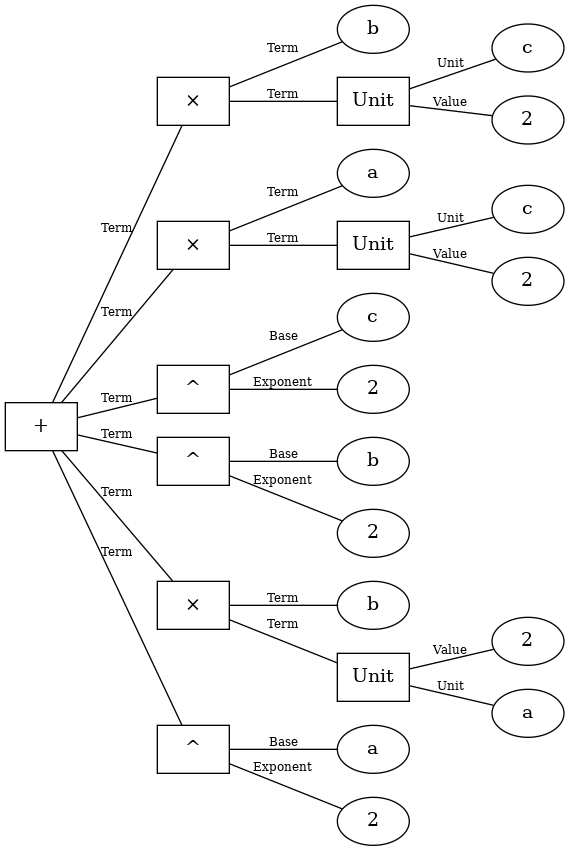
\includegraphics[width=0.5\textwidth]{image27}
  %\caption{Välj en olämplig bild}
\end{figure}
\newpage
\selectlanguage{english}
\begin{abstract}
The purpose of this project is to look at some of the techniques used by sites such as WolframAlpha to simplify algebraic expressions and solve particular kinds of equations. To research this we wrote an application in Python with some of the features of such sites.  We chose to work with Python because of how quickly code can be written in Python and due to the fact everybody in the group knew Python before the project even started. During the span of this project we were able to develop an application which is able to take input and construct an abstract syntax tree which is then simplified. The application is able to handle many of our goals set in the beginning, including addition and multiplication of polynomials correctly, although not always fully simplified. The application is also able to solve polynomials up to the second degree. With time the application could easily be expanded to cover more aspects of what we set out to do such as polynomial division and solving polynomial equations of higher grades.ga
\end{abstract}
\textbf{Keywords:} Abstract syntax tree; Python; Algebraic Expressions
\selectlanguage{swedish}
\end{document}
